\section{Kleene's Theorem}
\begin{theorem}
    Let \(A,B,B\) be sets such that \(A \subset B, B \subset C, C \subset A\).\\
    Then \(A=B=C\).
\end{theorem}
\begin{proof}
    Let \(x\) be an element of \(B\). \(x \in C\) (because \(B \subset C\)).
    Also \(x \in A\) (because \(C \subset A\)).
    Thus \(B \subset C\), and we can conclude \(A=B\).
    By analogy, \(B=C\) and thus all are equal.
\end{proof}
Regular expressions, finite automate, and transitions graphs each define a set of languages.
\begin{lemma}
    Every language that can be defined by a finite automaton can also be defined by a transition graph. \(FA \subset TG\)
\end{lemma}
\begin{proof}
    By definition (6.1), every finite automaton is itself already a transition graph.
    Therefore, any language that has been defined by an FA has already been defined by a TG.
\end{proof}
\begin{lemma}
    \label{lem:7.2}
    Every language that can be defined by a transition graph can also be defined by a regular expression. \(TG \subset RE\)
\end{lemma}
\begin{proof}
    By \textbf{constructive algorithm}, which works:
    \begin{enumerate}
            \item Add (if necessary) a unique start state without incoming edges and a unique final state without outgoing edges (connect with \(\Lambda\)).
            For each state repeat steps two and three.
            \item Use bypass and state elimination operation to reduce states.
            \item Combine edges that have the same starting and ending state.
            \item Combine edges from start and end state.
            The label on the only remaining edge is the regular expression result.
            If there is none, the regular expression is \(\Phi\).
        \end{enumerate}
\end{proof}
\newpage
\begin{example}
    This is a small example proving Lemma \ref{lem:7.2}.\\
    \begin{figure}[h!]
        \centering
        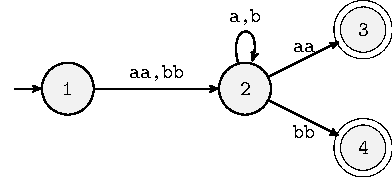
\includegraphics[width=0.5\linewidth]{lectures/figures/examples/7-1-1.pdf}
        \caption{Starting transition graph.}
    \end{figure}
    \begin{figure}[h!]
        \centering
        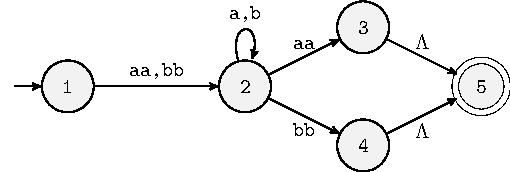
\includegraphics[width=0.6\linewidth]{lectures/figures/examples/7-1-2.pdf}
        \caption{Add final state 5 and remove acceptance from states 3 and 4.}
    \end{figure}
    \begin{figure}[h!]
        \centering
        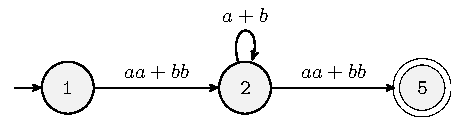
\includegraphics[width=0.6\linewidth]{lectures/figures/examples/7-1-3.pdf}
        \caption{Bypass states 3 and 4. Convert edges to regular expressions.}
    \end{figure}
    \begin{figure}[h!]
        \centering
        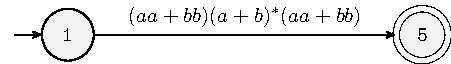
\includegraphics[width=0.6\linewidth]{lectures/figures/examples/7-1-4.pdf}
        \caption{Bypass state 2. Regular expression complete.}
    \end{figure}
    The final regular expression is: \((aa+bb)(a+b)^*(aa+bb)\).
\end{example}
\begin{lemma}
    Every language that can be defined by a regular expression can also be defined by a finite automaton. \(RE \subset FA\)
\end{lemma}
\begin{proof}
    \begin{enumerate}
        \item There is an FA that accepts only the empty word \(\Lambda\) and an FA that accepts only a single letter.
        \item If there is an FA that accepts the language defined by \(r_1\), and there is an FA that accepts the language defined by \(r_2\) then there is an FA that accepts the language \(r_1+r_2\).
        \item If there is an FA that accepts the language defined by \(r_1\), and there is an FA that accepts the language defined by \(r_2\) then there is an FA that accepts the language \(r_1r_2\).
        \item If there is an FA that accepts the language defined by \(r\) then there is an FA that accepts the language defined by \(r^*\).
    \end{enumerate}
    Thus for every regular expression, we can construct an FA.
\end{proof}

% continue here chapter 7 slide 32
% write RULES for lemma 7.3

\textbf{Kleene's Theorem} states that any language that can be defined by a regular expression, finite automaton, or transition graph can be defined by all three methods.